\graphicspath{{fig/introduction/}}

\chapter{Introduction}
\label{cha:introduction}

\section{Motivation}
\label{sec:motivation}

It is perfectly possible to live our everyday lives without giving a second
thought to the world around us. In fact, it can be rather easy to do so. Nature
becomes something secondary: an inconvenience of the past, something tamed by
modern amenity. But every once in a while comes an event which \emph{demands}
our attention. These displays of nature---the great ones---have the power to
invoke awe and wonder, offering a renewed appreciation of the natural world,
and our place within it.

One of these great displays of nature is represented by the collective motion
of animals. The canonical example of collective motion being the starling
murmuration (\cref{fig:murmuration}). In these events starlings gather 
in huge numbers and perform the most mesmerising of ballets; the entire flock
moving as if some fluid object. Coordinated, yet unpredictable, no two such
murmurations are ever the same. 

Another striking example of collective behaviour is given by the dense milling
structures sometimes formed by shoals of fish (\cref{fig:milling}). With these
structures the individuals form something greater than the sum of their parts:
their shoal taking on a life of its own. With a flash silver, and in the blink
of an eye, the shoal can change direction, offering an effective defence
against predation.

Collective motion, broadly defined as the formation of macro-level structures
from the interactions of individuals \parencite{camazine03}, has been observed
over many different length scales, and has been exhibited by many different
species \parencite{allee31}. But through all its variations and incantations,
the one thing that remains constant is the phenomenon's ability to capture the
attention and wonder of the observer.

\begin{figure}[t]
  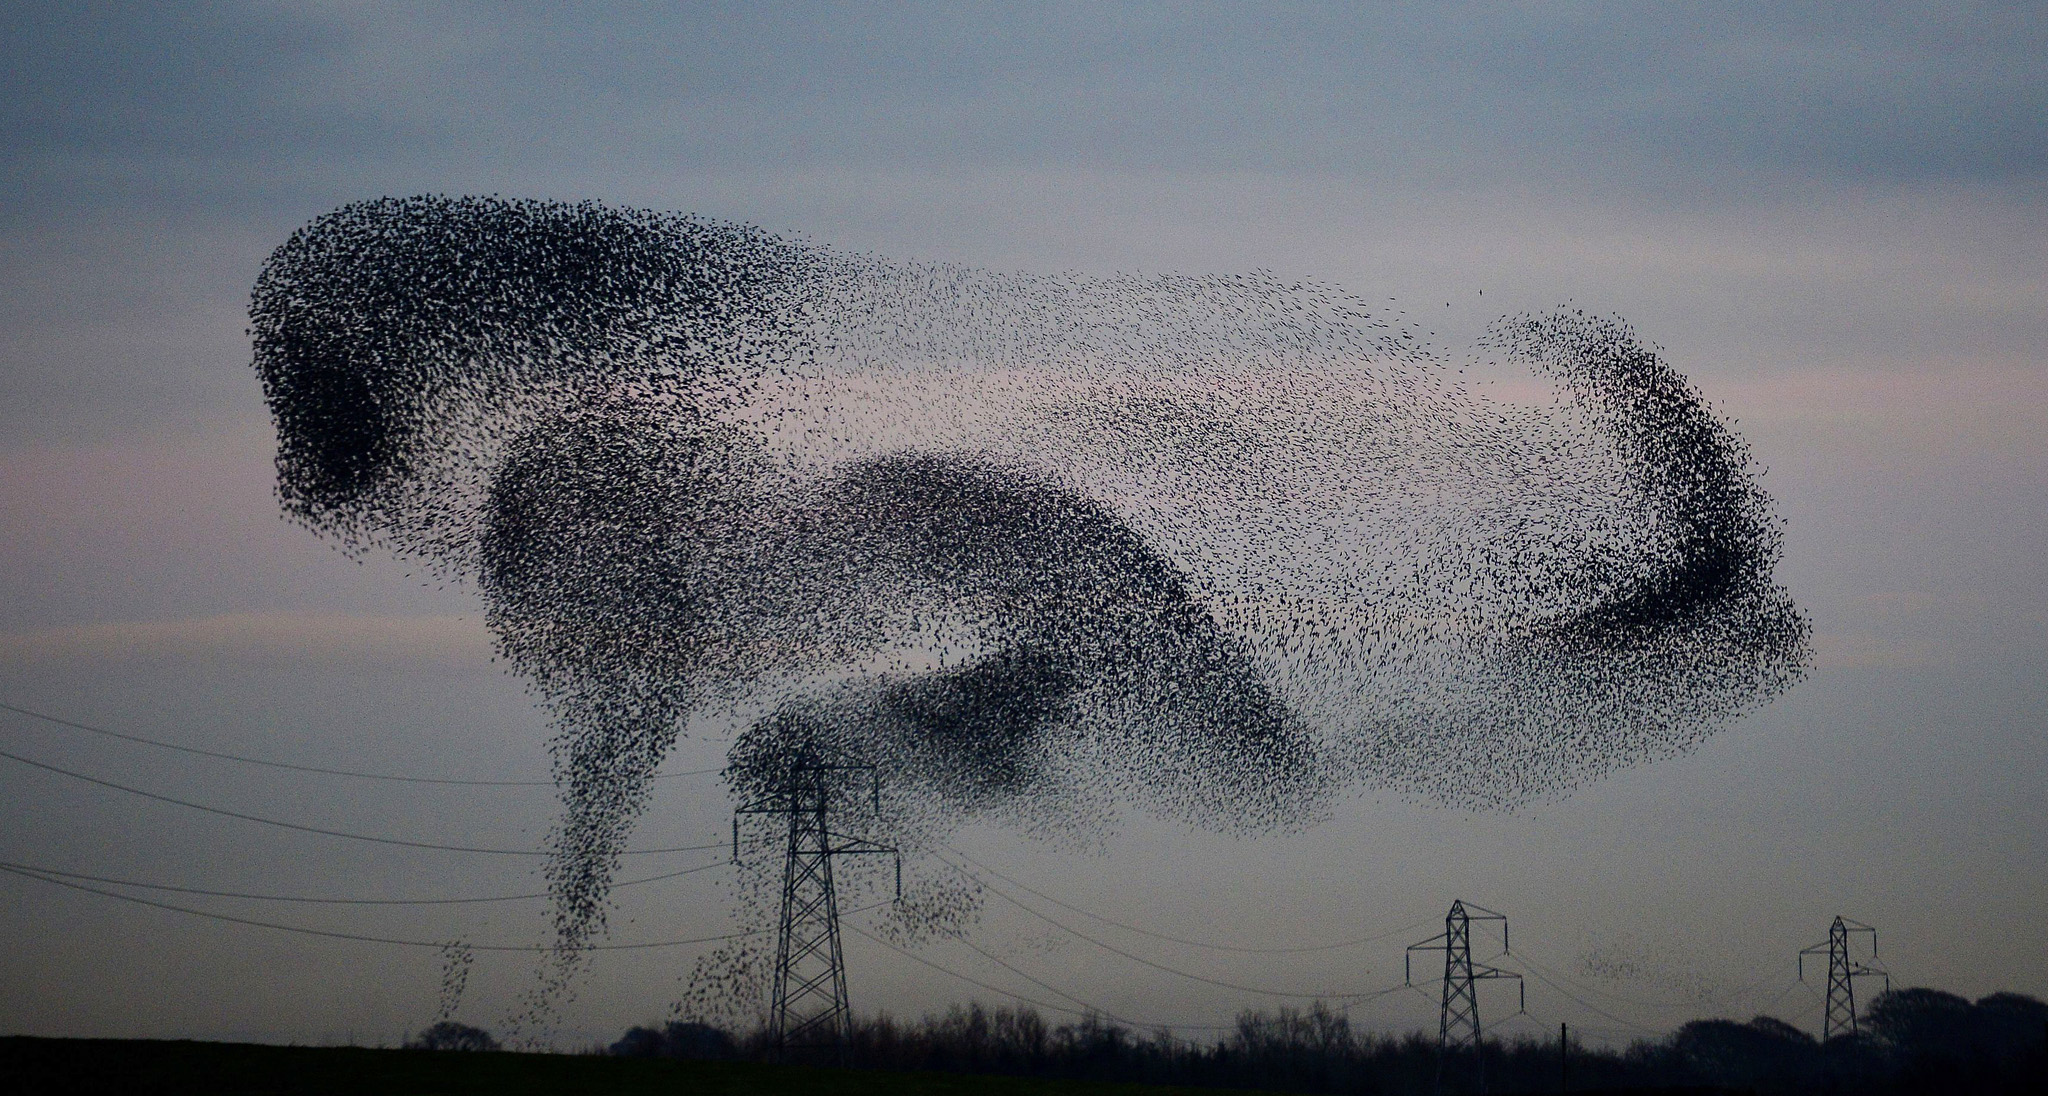
\includegraphics[width=\textwidth]{murmuration.jpg}
  \caption{A flock of starlings, here consisting of \emph{thousands} of
    individual members, gather to flock in the evening sky. These flocking
    events (often called murmurations), represent one of the most
    eye-catching displays of collective behaviour. This particular event
    was captured near Gretna, in the Scottish Borders. Photograph: Owen
    Humphreys/PA.}
  \label{fig:murmuration}
\end{figure}

Through captured imaginations, and over many years, collective behaviour has
become a thriving topic of multidisciplinary research, holding captive the
minds of physicists, biologists, mathematicians, and statisticians. Though our
understanding has evolved significantly from early suggestions that collective
behaviour results from thought-transference and telepathy between individuals
\parencite{selous31}, there is still much that remains unknown.

In many cases, the \emph{why} of collective behaviour is broadly understood.
From an evolutionary standpoint we can reason about the benefits which
collective behaviour brings to the individuals involved. For example, it is
known that aggregation can provide an effective defence against predation
\parencite{landeau86}, and that both foraging and migration can benefit from
the knowledge of the collective \parencite{simmons04}.

\begin{figure}[t]
  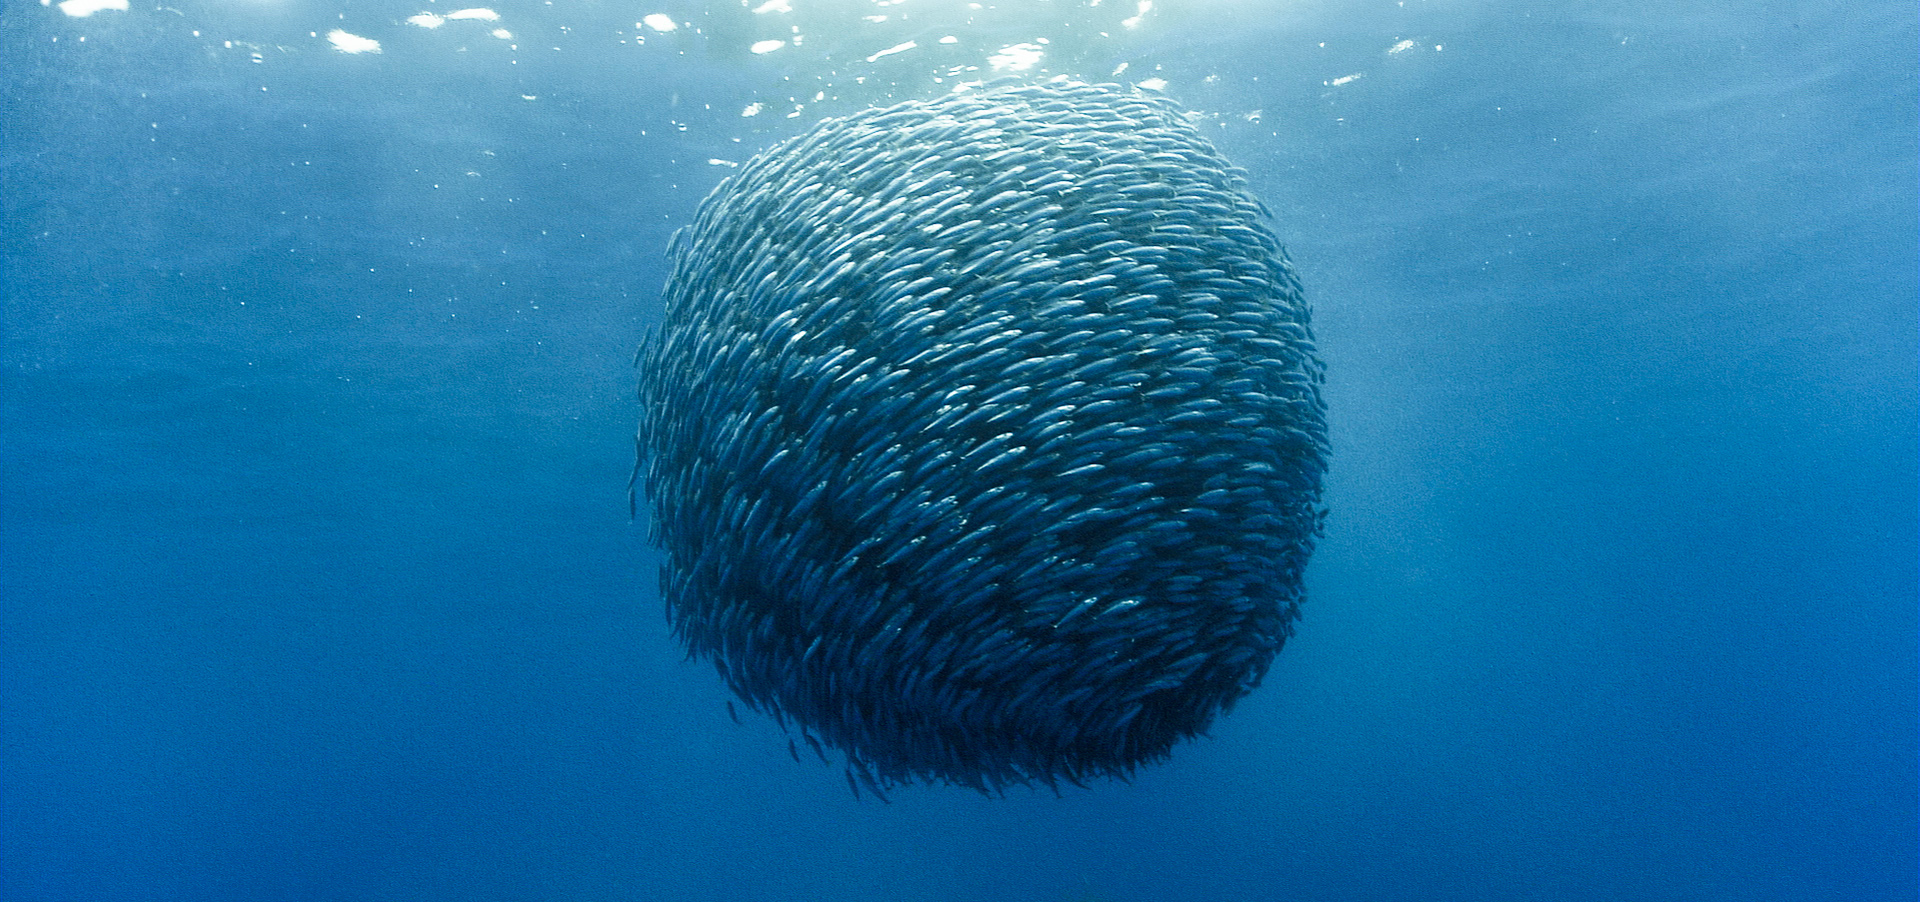
\includegraphics[width=\textwidth]{milling.jpg}
  \caption{Mackerel forming a tight milling structure in open water. The
    individuals behave as one entity, and can swell, change direction,
    deform and reform in fractions of a second. These structures form
    spontaneously in the presence of danger, and act as a defence against
    predation.}
  \label{fig:milling}
\end{figure}

Despite this, much less is known about the \emph{how} of collective behaviour.
The mechanisms which lead to the formation and maintenance of aggregations
remain elusive, and are a topic of much continued interest. The hope is that
the study of mathematical models of flocking, and the comparison of these
models with real flocking events, will lead to insights about the mechanics
which underlie these phenomena. In recent years modern computing has made the
process of simulating such models (relatively) pain-free. However, a lack of
data describing real flocking events has made the comparison between model and
data difficult.

Previously, much work has been invested in developing the theoretical models
which seek to explain emergent behaviour by interactions at an individual
level. Such models have shown that individual interactions are sufficient to
produce group-level structures \parencite{aoki82}. Many different simulations,
implementing disparate interaction rules, are able to produce behaviour
reminiscent of real flocking systems. However, these models have largely only
been verified with comparison to empirical observation at a qualitative level,
and thorough quantitative comparison between data and theory has been lacking.
The lack of quantitative comparison between model and data can largely be
attributed to the scarcity of appropriate empirical data.

However, in recent years technological and methodological advances have made it
possible to capture the movements of large groups of animal aggregations
\parencite{ballerini08}. With this data, it is only now that we are in a
position to make robust comparison between model prediction and real-world
observation.

This thesis considers and develops theoretical models of collective behaviour
popular in the literature. This development is guided by considerations of
biological realism. Simulation studies are performed which show that the
developed models can be fit to simulated data, after which the same models are
fit to real data. The efficacy of each fitted model is compared, and a subclass
of the candidate models are presented as providing the best fit.

\section{Thesis overview}
\label{sec:overview_of_thesis}

In \cref{cha:lit_review} the reader is given a review of the literature
surrounding the study of collective behaviour. Important ideas and results of
the field are introduced, summarised and discussed. After relaying the main
results from the literature, open problems and the future of research
in the field are discussed.

Bayesian statistics is introduced to the reader in \cref{cha:bayes_intro}. The
underlying philosophy of the Bayesian paradigm, as well as important results,
techniques and algorithms are outlined. Consideration is given for common
problems that the Bayesian practitioner may encounter, as well as how one might
address these problems.

In the proceeding chapter, \cref{cha:model_dev}, a class of model popular in
the literature of collective behaviour is introduced. The short-comings of this
model are then considered and summarised, and alterations are proposed to
address the short-comings. The proposed changes are motivated by considerations
of biological-realism.

Following on from this, \cref{cha:sim_studies} details the results of a number
of so-called simulation studies. In these studies a model is forward simulated
for known parameter values. A practitioner is then tasked with capturing these
known parameter values with statistical inference. A number of simulation
studies are performed on variations of a previously considered model.

The statistical machinery built in \cref{cha:sim_studies} is then repurposed in
\cref{cha:sheep}, as our developed models are fit to real observations. Fitting
a number of different models to the same data, the predictive performance of
these models are compared, and a subclass of these models are identified as
providing the best fit.

\cref{cha:missing} considers the problem of missing data. It is argued that the
nature of flocking events means that missing data becomes an inevitable issue.
Algorithms are outlined which allow the scientist to account for additional
uncertainty introduced by missingness. Proof-of-concept is shown by performing
simulation studies on data with artificially imposed missingness.

In \cref{cha:scoters} a dataset of a real flocking event with missing
observations is introduced. The limitations of previous studies of this data
are outlined. The analysis presented in this thesis addresses the short-comings
of previous work, accounting for the additional uncertainty introduced by the
missing observations.

For the uninitiated, a review of circular statistics is presented in
\cref{cha:direct_stats}. This review motivates the study of circular
statistics, and argues it relevance to the scientist involved in the study of
collective behaviour.
